\begin{frame}{Examples of Featureless Insulators}
\vskip-1.5cm
			
\begin{columns}[T]
\begin{column}[T]{.5\textwidth}
		\begin{block}{Classical Insulators}
			\vskip-0.3cm
	  	\begin{figure}
				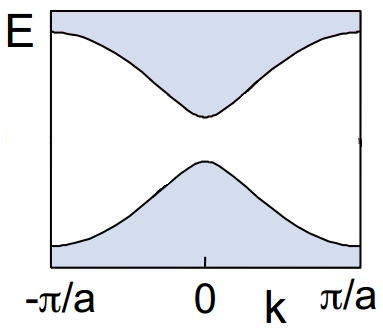
\includegraphics[width=0.5\linewidth]{diagrams/band_insulator_2.png}
				\caption{Free fermion band insulator}
			\end{figure}
			\begin{figure}
			\vskip-0.6cm
				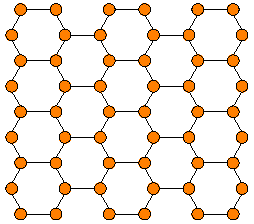
\includegraphics[width=0.5\linewidth]{diagrams/filled_honeycomb.pdf}
				\caption{Atomic picture}
				%Some integer number of localized orbitals filled, integer charge per site
			\end{figure}
		\end{block}
\end{column}
\begin{column}[T]{.5\textwidth}
	\begin{block}{Topological Insulators}
		\vskip-0.3cm
		\begin{figure}
			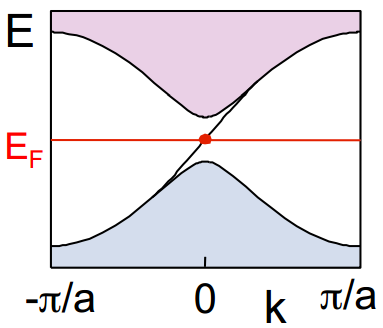
\includegraphics[width=0.5\linewidth]{diagrams/chiral_edge.png}
			\caption{Band insulator with chiral edge}
			%Not viewed as some integer number of orbitals filled per unit cell
		\end{figure}
		\begin{figure}
			\vskip-0.7cm
				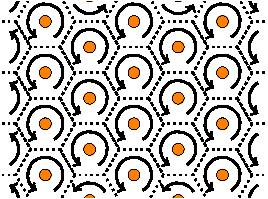
\includegraphics[width=0.5\linewidth]{diagrams/honeycomb_breakdown.pdf}
				\caption{Atomic picture breaks down}
		\end{figure}
	\end{block}

\end{column}
\end{columns}

\end{frame}

%Examples include free fermion band insulators, both trivial and topological
%Interacting 1D examples would include the spin-1 heisenberg AFM